\subsection{UC-4}

\begin{figure}[H]
    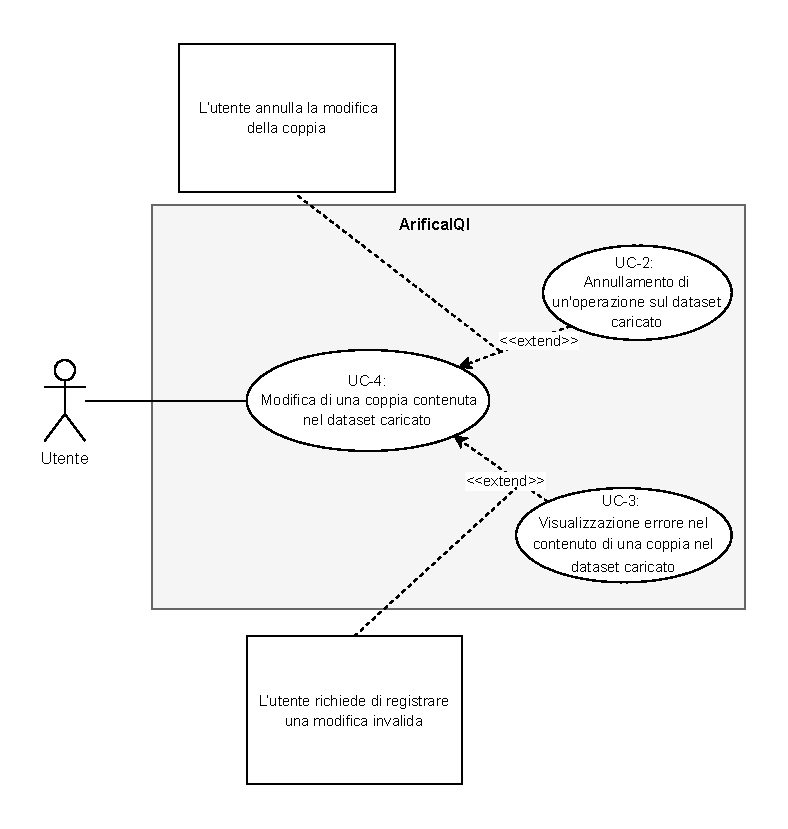
\includegraphics[scale=0.8]{Sezioni/UseCase/Immagini/UC-4.pdf}
    \caption{Diagramma UC-4.}
\end{figure}

\begin{usecase}{UC-4}{Modifica di una coppia contenuta nel dataset corrente}
    
    \req{\hyperref[item:RU-1]{RU-1}} 

    \pre{
        \item Il sistema è attivo e funzionante
        \item Il dataset corrente non è vuoto
        \item La coppia da modificare esiste
    }

    \post{
        \item La coppia viene aggiornata
        \item Il dataset corrente viene aggiornato
    }
    
    \actor{Utente}

    \subactors{}

    \trigger{L'utente deve modificare una coppia contenuta nel dataset corrente}
    
    \inc{}

    \base{}

    \scenario{
        \item L'utente richiede la modifica di una coppia
        \item L'utente modifica il contenuto della coppia
        \item L'utente conferma la modifica della coppia
        \item La coppia viene aggiornata nel dataset corrente

    }

    \subscenario{
        \item[2.1] \textbf{L'utente annulla la modifica della coppia} 
        \begin{itemize}
            \item[a.] \hyperref[subsec:UC-2]{UC-2}
        \end{itemize}
        \item[3.1] \textbf{L'utente richiede di registrare una modifica invalida}
        \begin{itemize}
            \item[a.] \hyperref[subsec:UC-3]{UC-3}
        \end{itemize}
    }
\end{usecase}
